\documentclass[hidelinks]{article}

%%%%%%%%%%%%%%%%%%%%%%%%%%%%%%%%%%%%%%%%%%%%%%%%%%%%%%%%%%%%%%%
% START CUSTOM INCLUDES & DEFINITIONS
%%%%%%%%%%%%%%%%%%%%%%%%%%%%%%%%%%%%%%%%%%%%%%%%%%%%%%%%%%%%%%%
\usepackage{amsmath,amssymb,amsfonts,amsthm}
\usepackage{parskip} %noident everywhere
\usepackage{mathtools}
\usepackage{subcaption}
\usepackage{overpic}
\usepackage{mymath}
\usepackage{nth}
\usepackage{caption}
\usepackage{todonotes}
% \usepackage{fullpage} % Hidden if footers
\usepackage{arydshln} % dashed line in array
\usepackage{MnSymbol} % anti-diag dots
%\usepackage{showlabels} % show equation and figure labels
\usepackage{hyperref} % Show hyperlinks - claudio
\hypersetup{
    colorlinks = true
    linkcolor = blue
    urlcolor = red
    pdftitle = Dykstra - Claudio
    }
\usepackage{fancyhdr, lastpage} % Headers and footers
\pagestyle{fancy}
\lhead{2024}
\rhead{Claudio Vestini \& Idris Kempf} % hidden if full page
\cfoot{Page \thepage\ of \pageref{LastPage}}
\usepackage{subcaption}
\usepackage{varwidth, tikz}
\usetikzlibrary{shapes, arrows, shapes.misc, arrows.meta, positioning, matrix, calc, fit, fadings, patterns}
\usetikzlibrary{calc,patterns,decorations.pathmorphing,decorations.markings,arrows, arrows.meta}
\usepackage[export]{adjustbox}
\usepackage{placeins}
% \setlength{\parindent}{0pt} % no indent, more aggressive
\usepackage{tabto}

\newtheorem{lemma}{Lemma}
\newtheorem{definition}{Definition}
\newtheorem{theorem}{Theorem}
\newtheorem{corollary}{Corollary}
\newtheorem{proposition}{Proposition}
\newtheorem{assumption}{Assumption}

%%%%%%%%%%%%%%%%%%%%%%%%%%%%%%%%%%%%%%%%%%%%%%%%%%%%%%%%%%%%%%%
% END CUSTOM INCLUDES & DEFINITIONS
%%%%%%%%%%%%%%%%%%%%%%%%%%%%%%%%%%%%%%%%%%%%%%%%%%%%%%%%%%%%%%%

\pdfobjcompresslevel=0

\title{Dykstra's Algorithm for Projection onto Convex Sets: Stalling Analysis}
\author{Claudio Vestini and Idris Kempf}
\date{September 2024}
\begin{document}
\maketitle
%
\section{Context \& Background}
The forthcoming upgrade of the Diamond Light Source (DLS) synchrotron presents a complex control challenge in the stabilisation of the electron beam. This is due to the increased number of sensors (from 172 to 252) and actuators (from 173 to 396), as well as the introduction of two different types of corrector magnets~\cite{MPCDLSII}. Traditional control methods (\textit{modal decomposition}~\cite{HEATH}) are no longer sufficient, and model predictive control (MPC), while promising, faces high computational demands for high-frequency (100 kHz) control. The optimiser has to solve a constrained quadratic programming (CQP) problem at each timestep in less than $10\mu\!\text{s}$ for feasibility. This involves minimising a cost function to obtain a global minimum, and projecting it onto the constraint set. The projection step can be solved using Dykstra's method~\cite{DYKSTRA}, which has been shown to converge linearly~\cite{DYKSTRAPOLY2}. 
% RE-WRITE THIS LATER
This algorithm can stall under certain conditions~\cite{DYKSTRASTALLING}, and this paper will investigate stalling and how it may be prevented.
%
\section{Problem Statement}
The relationship between the $n_y = 252$ measured beam displacements $\inRv{{y}_k}{n_y}$ and the $n_u = 396$ actuator inputs $\inRv{{u}_k}{n_u}$ can be described by the state-space representation of a linear system in discrete time,
\begin{subequations}
\begin{align}\label{eq:statespace}
{x}_{k+1}&={A}{x}_{k}+{B}{u}_{k},\quad u_k\in\mathcal{U}({u}_{k\sm 1}),\\
{y}_{k}&={C}{x}_{k}+{d}_{k},
\end{align}
\end{subequations}
where $\inRv{{x}_k}{n_x}$ are the states at time $t=k T_s$. The inputs ${u_k}$ are subjected to amplitude and slew-rate constraints that can be modelled as $\mathcal{U}({u}_{k\sm 1})\eqdef\mathcal{A}\cap\mathcal{R}({u}_{k\sm 1})$, where ${u}_{k\sm 1}$ is the input applied at time $t=(k-1) T_s$ and $\mathcal{A}$ and $\mathcal{R}({u}_{k\sm 1})$ are the amplitude and slew-rate constraint sets:
\begin{subequations}\label{eq:constraints}
\begin{align}
\mathcal{A}&\eqdef\set{{u}_{k}\in\R^{n_u}}{-\alpha \leq {u}_{k} \leq \alpha},\\
\mathcal{R}({u}_{k\sm 1})&\eqdef\set{{u}_{k}\in\R^{n_u}}{-\rho \leq {u}_{k}\sm {u}_{k\sm 1} \leq \rho}.
\end{align}
\end{subequations}

The condensed~\cite{MPCBOOK} model predictive control problem for~\eqref{eq:statespace} is
\begin{align}\label{eq:qpshort}
\min_{{u}} \frac{1}{2}\trans{{u}}{J}{u}+\trans{{q}({\hat{x}}_k, {\hat{d}}_k)}{u}\quad\text{s.t.}\quad{u}\in\mathcal{S}({u}_{\sm 1}),
\end{align}
where ${u}\eqdef({u}_0^\Tr,\dots,{u}_{N\sm 1}^\Tr)^\Tr\!\in\!\R^{Nn_u}\!$, $N$ the horizon, $f(u)\eqdef\frac{1}{2}\trans{{u}}{J}{u}+\trans{{q}({\hat{x}}_k, {\hat{d}}_k)}{u}$ the objective function and $\inR{{J}=\trans{{J}}}{Nn_u}{Nn_u}$ the Hessian. The vector ${q}({\hat{x}}_k, {\hat{d}}_k)$ is an affine function of the observer output ${\hat{x}}_k$ and ${\hat{d}}_k$. The closed convex set $\mathcal{S}({u}_{\sm 1})$ is defined as
\begin{align}\label{eq:set}
\mathcal{S}({u}_{\sm 1})\eqdef\mathcal{U}({u}_{\sm 1})\times\dots\times\,\mathcal{U}({u}_{N\sm 2}),
\end{align}
and depends on the input ${u}_{\sm 1}$ applied at time $t-1$. The following assumptions on problem~\eqref{eq:qpshort} are made throughout the paper: 
\newtheorem*{ass1}{Assumption I.a}
\begin{ass1}[Strong convexity]
It holds that $0\prec \lambda_\text{min}I\preceq J\preceq\lambda_\text{max}I$, where $\lambda_\text{min}$ and $\lambda_\text{max}$ are the minimum and maximum eigenvalues of $J$. 
\end{ass1}
\newtheorem*{ass2}{Assumption I.b}
\begin{ass2}[Bounded inputs]
The set $\mathcal{S}$ is bounded, so that $\abs{\mathcal{S}}\eqdef \max_{x,y\in\mathcal{S}}\,\twonorm{x-y}<\infty$.
\end{ass2}

To solve problem~\eqref{eq:qpshort}, we are using the fast gradient method~\cite{FGMDYKSTRAARXIV}. The present variant of the fast gradient method is applicable to strongly convex functions for ill-conditioned Hessians~\cite[Ch. 2.2.4]{OPTIMNESTEROV}. The fast gradient method requires the Hilbert space projection $\mathcal{P}_{\mathcal{S}}$ onto $\mathcal{S}$, and no simple formula exists for $N>1$. Here, we are replacing the exact projection $\mathcal{P}_{\mathcal{S}}$ with Dykstra's alternating projection algorithm, $\mathcal{D}_{\mathcal{S}}$. Dykstra's method is an iterative algorithm that yields the exact projection if the algorithm is run for an infinite number of iterations. For $M$ iterations, $\mathcal{D}_\mathcal{S}(z)\not\in\mathcal{S}$ in general\footnote{For example, consider the projection onto a corner (or edge) of two intersecting hyperplanes.} and the method yields a projection error that can be quantified as shown in the following assumption.
\newtheorem*{ass3}{Assumption II}
\begin{ass3}[Approximate projection]
Dykstra's method $\mathcal{D}_{\mathcal{S}}$ returns a point $\mathcal{D}_{\mathcal{S}}(z)$ that satisfies
\begin{align}
\twonorm{\mathcal{D}_{\mathcal{S}}(z) - \mathcal{P}_{\mathcal{S}}(z)} \leq \delta (z,M,\mathcal{S}),
\end{align}
where the upper bound $\delta (z,M,\mathcal{S})>0$ depends on the maximum number of iterations $M$ of Dykstra's method.
\end{ass3}
We wish to characterize $\delta (z,M,\mathcal{S})$ for $\mathcal{S}$ and $z\in\mathcal{Z}$, where $\mathcal{Z}=\mathcal{Z}(J,q,u_{\sm 1})$ is to be defined.
\newpage
%
\section{Dykstra's Alternating Projection}
% Claudio's contribution
The projection step of the fast gradient method can be solved using Dykstra's algorithm.
Given $n$ convex sets $\mathcal{H}_1,\dots,\mathcal{H}_n$, Dykstra's alternating projection algorithm~\cite{DYKSTRAPERKINS} finds the orthogonal projection $x^\star$ of $x$ onto $\mathcal{H}\eqdef{\bigcap}_{i=1}^n \mathcal{H}_i$ by initially setting
%
% I changed the citation paper as this one has much more intuitive notation
\begin{align}\label{eq:initial error}
&e_{-n} = e_{-(n-1)} = ... = e_{-1} = \vec0
\end{align}
and generating a series of iterates \{$x_{m}$\} using the scheme
\begin{align}\label{eq:dykstra}
&x_{m+1}=\mathcal{P}_{\mathcal{H}_{[m]}}\left(x_{m}+e_{m-n}\right),
&e_m=x_{m}+e_{m-n}-x_{m+1},
\end{align}
for $[m]= 0,1,...$ and $x_0=x$.
%
\newline
This is a variation of the simpler Von Neumann's \emph{Method of Alternating Projections} (MAP), which can be obtained from (\ref{eq:dykstra}) with the errors $e_m = \vec0$. A visual explanation of the difference between the two methods is displayed in Figure~\ref{fig:wiki}
%
% Figure demonstrating both methods (from Wikipedia)
\begin{figure}[h]
    \centering
    
    \begin{subfigure}[t]{0.49\textwidth}
        \centering
        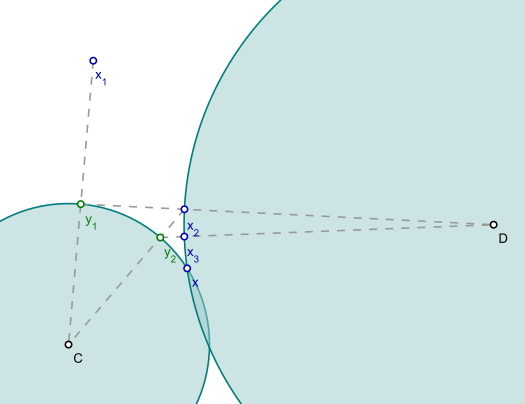
\includegraphics[width=1\textwidth]{Latex/Current Version/Figures/MAP_wiki.png}
        \caption{MAP algorithm with successive projections y and x onto sets C and D respectively}
        \label{fig:wikiMAP}
    \end{subfigure}
    \hfill
    \begin{subfigure}[t]{0.49\textwidth}
        \centering
        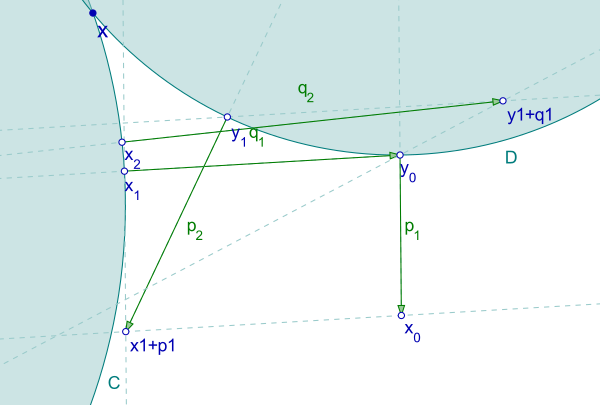
\includegraphics[width=1\textwidth]{Latex/Current Version/Figures/Dykstra_wiki.png}
        \caption{Dykstra's algorithm with associated errors p and q}
        \label{fig:wikiDykstra}
    \end{subfigure}
    \caption{A demonstration of MAP vs Dykstra. Dykstra has intermediate steps}
    \label{fig:wiki}
\end{figure}
%
\newline
Despite MAP being much simpler, it exhibits weak convergence~\cite{BREGMAN} and does not always produce an optimal output, as illustrated in Figure~\ref{fig:demonstration}.
%
% Figure demonstrating sub-optimality of MAP
\begin{figure}[h]
    \centering
    
    \begin{subfigure}[t]{0.49\textwidth}
        \centering
        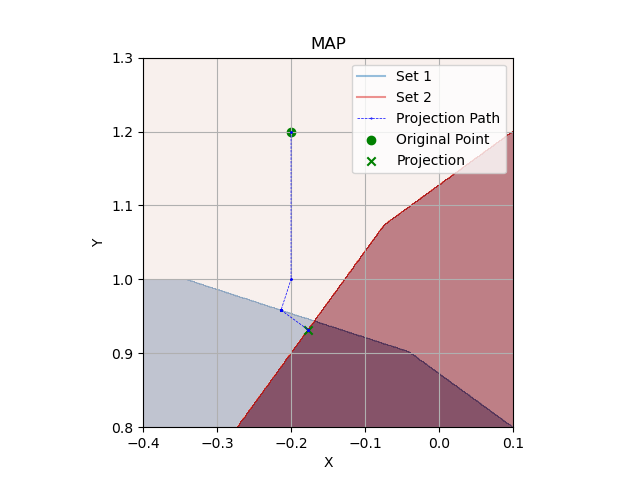
\includegraphics[width=1\textwidth]{Latex/Current Version/Figures/MAP_demonstration.png}
        \caption{Sub-optimal solution for MAP after 1 iteration. Nothing happens in second iteration}
        \label{fig:demonstrationMAP}
    \end{subfigure}
    \hfill
    \begin{subfigure}[t]{0.49\textwidth}
        \centering
        \includegraphics[width=1\textwidth]{Latex/Current Version/Figures/Dykstra_demonstration.png}
        \caption{Dykstra gets closer to optimal solution in second iteration}
        \label{fig:demonstrationDykstra}
    \end{subfigure}
    \caption{A demonstration of solution optimality. Both algorithms were ran for two iterations. Dykstra's will produce an optimal output after infinitely many iterations}
    \label{fig:demonstration}
\end{figure}
%
\par The Boyle-Dykstra theorem~\cite{DYKSTRA} implies that $\lim_{m\rightarrow\infty}\anynorm{x_m-\mathcal{P}_\mathcal{H}(x)}=\vec0$. For a finite number of iterations, there is no guarantee that $x_m\in\mathcal{H}$. 
%
\newpage
Here, we assume that $\mathcal{H}$ is a polyhedron and the $\mathcal{H}_i$ are halfspaces given by
\begin{align}\label{eq:sets_i}
\mathcal{H}_i\eqdef\set{x}{\iprod{x}{f_i} \leq c_i},
\end{align}
where $\anynorm{f_i}=1$. In addition, define boundaries
\begin{align}\label{eq:sets_i2}
H_i\eqdef\set{x}{\iprod{x}{f_i} = c_i},
\end{align}
so that $\text{int}\,\mathcal{H}_i\eqdef\mathcal{H}_i\backslash H_i$. The projections onto $H_i$ and $\mathcal{H}_i$ are given by
\begin{align}
&\mathcal{P}_{H_i}(x)=x-\left(\iprod{x}{f_i} - c_i\right)f_i,
&\mathcal{P}_{\mathcal{H}_i}(x)=\begin{cases}
x & \text{if } x\in\mathcal{H}_i\\
\mathcal{P}_{H_i}(x) & \text{if } x\not\in\mathcal{H}_i\,.
\end{cases}
\end{align}
For this particular choice of sets, $e_m = k_m f_{[m]}$ with $k_m=\text{dist}_{\mathcal{H}_{[m]}}(x_{m-1}+e_{m-n})$, i.e. the auxiliary vector is either $0$ or parallel to $f_{[m]}$. 
%
The convergence of Dykstra's method has been analyzed in~\cite{DYKSTRAPOLY2,DYKSTRAPOLY}, where it has been shown that the convergence is linear. In~\cite{DYKSTRAPOLY}, the proof is based on partitioning the set $\lbrace 1,\dots,n\rbrace$ into
\begin{align}
&A=\set{i\in\lbrace 1,\dots,n\rbrace}{x_\infty\in H_i},
&B=\lbrace 1,\dots,n\rbrace\backslash A=\set{i\in\lbrace 1,\dots,n\rbrace}{x_\infty\in\text{int}\,\mathcal{H}_i},
\end{align}
where $x_\infty=\lim_{m\rightarrow\infty}x_m$. It can be shown that there exists a number $N_1$ such that whenever
\begin{align}
[m]\in B,\quad m\geq N_1\quad\Rightarrow\quad x_m=x_{m-1},\quad e_m=\vec0,
\end{align}
i.e. the half-spaces in $B$ become ``inactive''. Furthermore, there exists $N_2\geq N_1$ such that whenever $n\geq N_2$, it holds that
\begin{align}
\twonorm{x_{m+n}-x_\infty}\leq\alpha_{[m]}\twonorm{x_m-x_\infty},
\end{align}
where $0\leq\alpha_{[m]}<1$. With these ingredients, the following result is obtained:
\begin{theorem}
There exist constants $0\leq c < 1$ and $\rho > 0$ such that
\begin{align*}
\anynorm{x_m -x_\infty} \leq \rho c^m.
\end{align*}
\end{theorem}
The factor $c$ can be estimated from the smallest $\alpha_{[m]}$, which is characterized by the angle between certain subspaces (subspaces formed by the ``active'' halfspaces). The factor $\alpha_{[m]}$ can be upper-bounded by considering the ``worst'' angles in the polyhedron.
%
The constant $\rho$, however, depends on a number $N_3\geq N_2$ and on $x$. It is unclear how to obtain that constant $\rho$. In fact, the authors of~\cite{DYKSTRAPERKINS} and~\cite{XUPOLY} emphasize that $\rho$ cannot be computed in advance, and that the inability to compute a bound on the projection error makes the application of Dykstra's method difficult. The authors of~\cite{DYKSTRAPERKINS} proposed a combined Dysktra-conjugate-gradient method that allows for computing an upper bound on $\anynorm{x_m -x_\infty}$. The authors of~\cite{XUPOLY} proposed an alternative algorithm called \emph{successive approximate algorithm}, which promises fast convergence, conditioned on knowing a point $x\in\mathcal{H}$ in advance. \label{sec: dykstra}
%
\section{Stalling}
%
In~\cite{DYKSTRASTALLING}, the behaviour of Dykstra's method is analysed for two sets. The authors give conditions on Dykstra's algorithm for (1) finite convergence, (2) infinite convergence and (3) stalling followed by infinite convergence. 
%
A specific example is given for the case that the set is provided by the intersection of a line with a unit box in $\R^2$ ($\mathcal{H}$ is a polyhedron). It can be shown that cases (1)--(3) depend on the starting point $x_0$, and one can determine the 3 regions shown in Figure~\ref{fig:region} that yield different convergence behaviour. Convergence case 1 is obtained when starting in the green region, case 2 when starting in the blue region and case 3 when starting in the red region.
%
\par To understand the stalling effect, consider Figure~\ref{fig:stalling}, which shows the first iterations of Dykstra's algorithm with starting point in the red region. Note that the outcome of Dykstra's algorithm depends on the order of the sets $\mathcal{H}_i,\dots,\mathcal{H}_n$. In Figure~\ref{fig:stalling}, the algorithm starts by projecting onto the box and then onto the line. It can be seen that for the first 6 iterations\footnote{By one iteration we mean one cycle of $n$ projections here.}, Dykstra's algorithm returns the top left corner of the box (``stalling''). The authors also determine the exact number of iterations required to break free from the red region, and show that if the starting point is arbitrarily far to the left, the algorithm will need an arbitrarily large iteration number to break free from the red region.
%
% Figure demonstrating the stalling problem
\begin{figure}[h]
    \centering
    
    \begin{subfigure}[t]{0.49\textwidth}
        \centering
        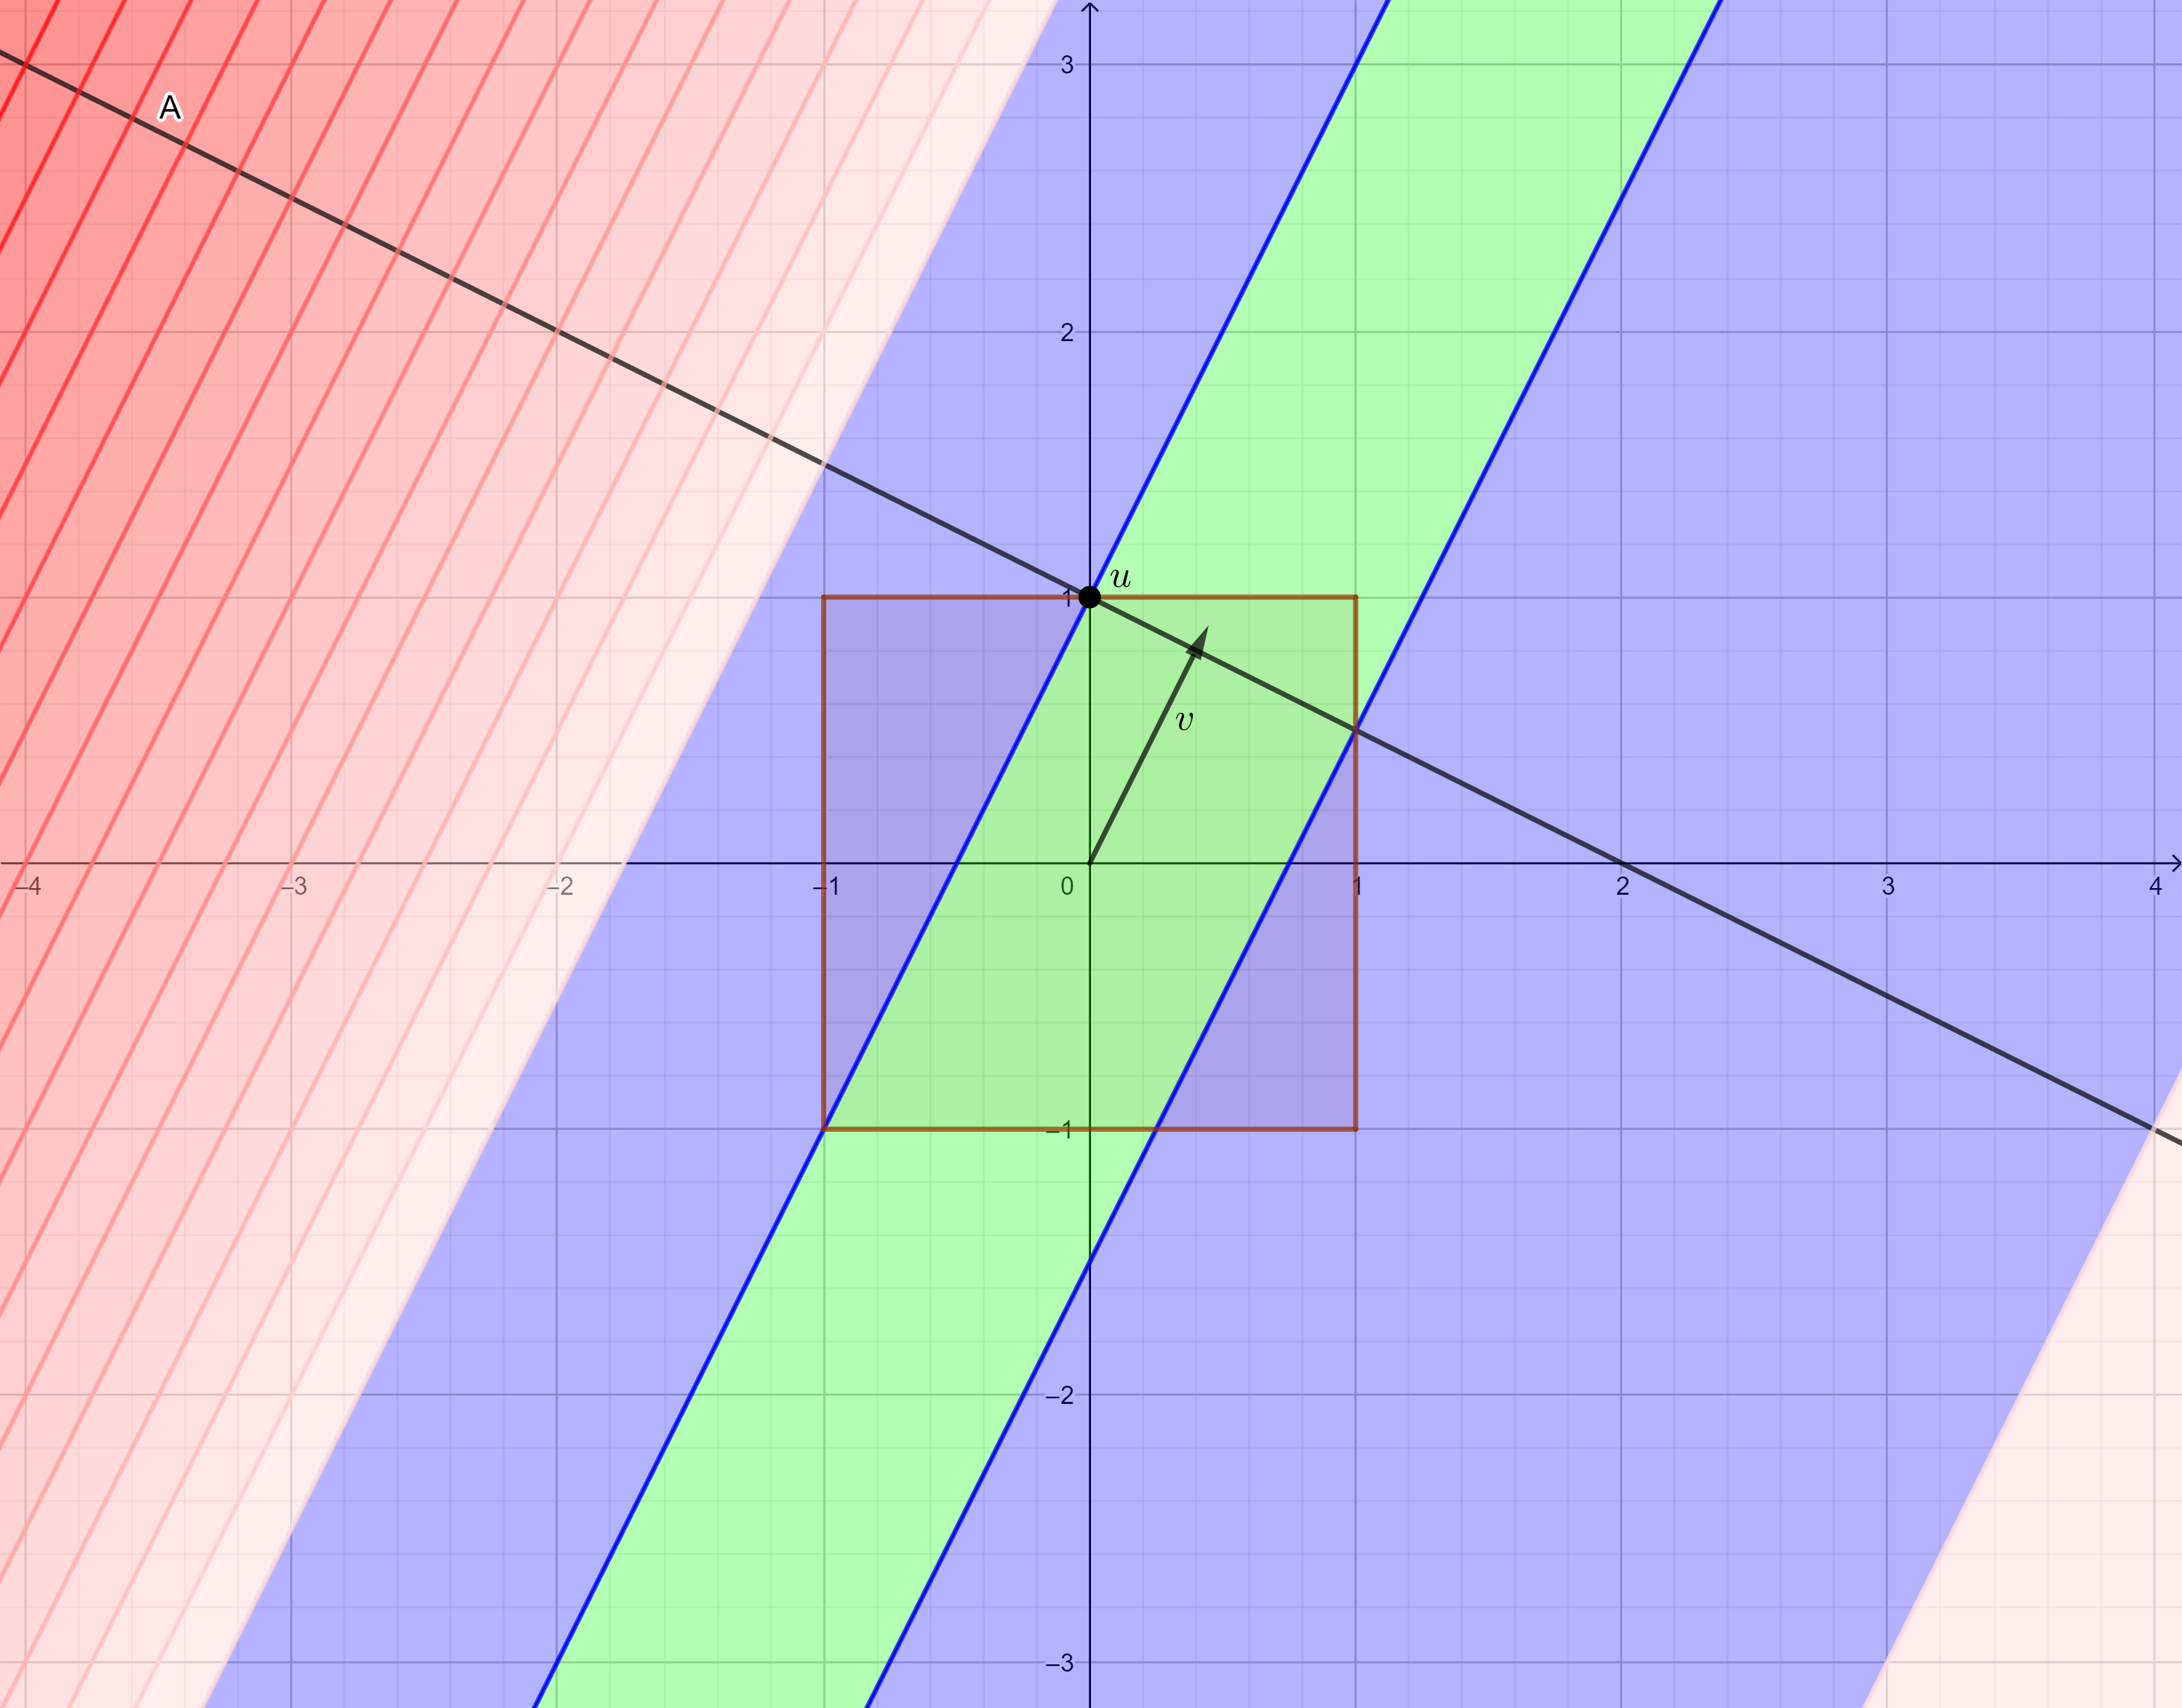
\includegraphics[width=1\textwidth]{Latex/Current Version/Figures/StallingRegionsHand.png}
        \caption{Line-box example with different regions that yield different convergence properties.}
        \label{fig:region}
    \end{subfigure}
    \hfill
    \begin{subfigure}[t]{0.49\textwidth}
        \centering
        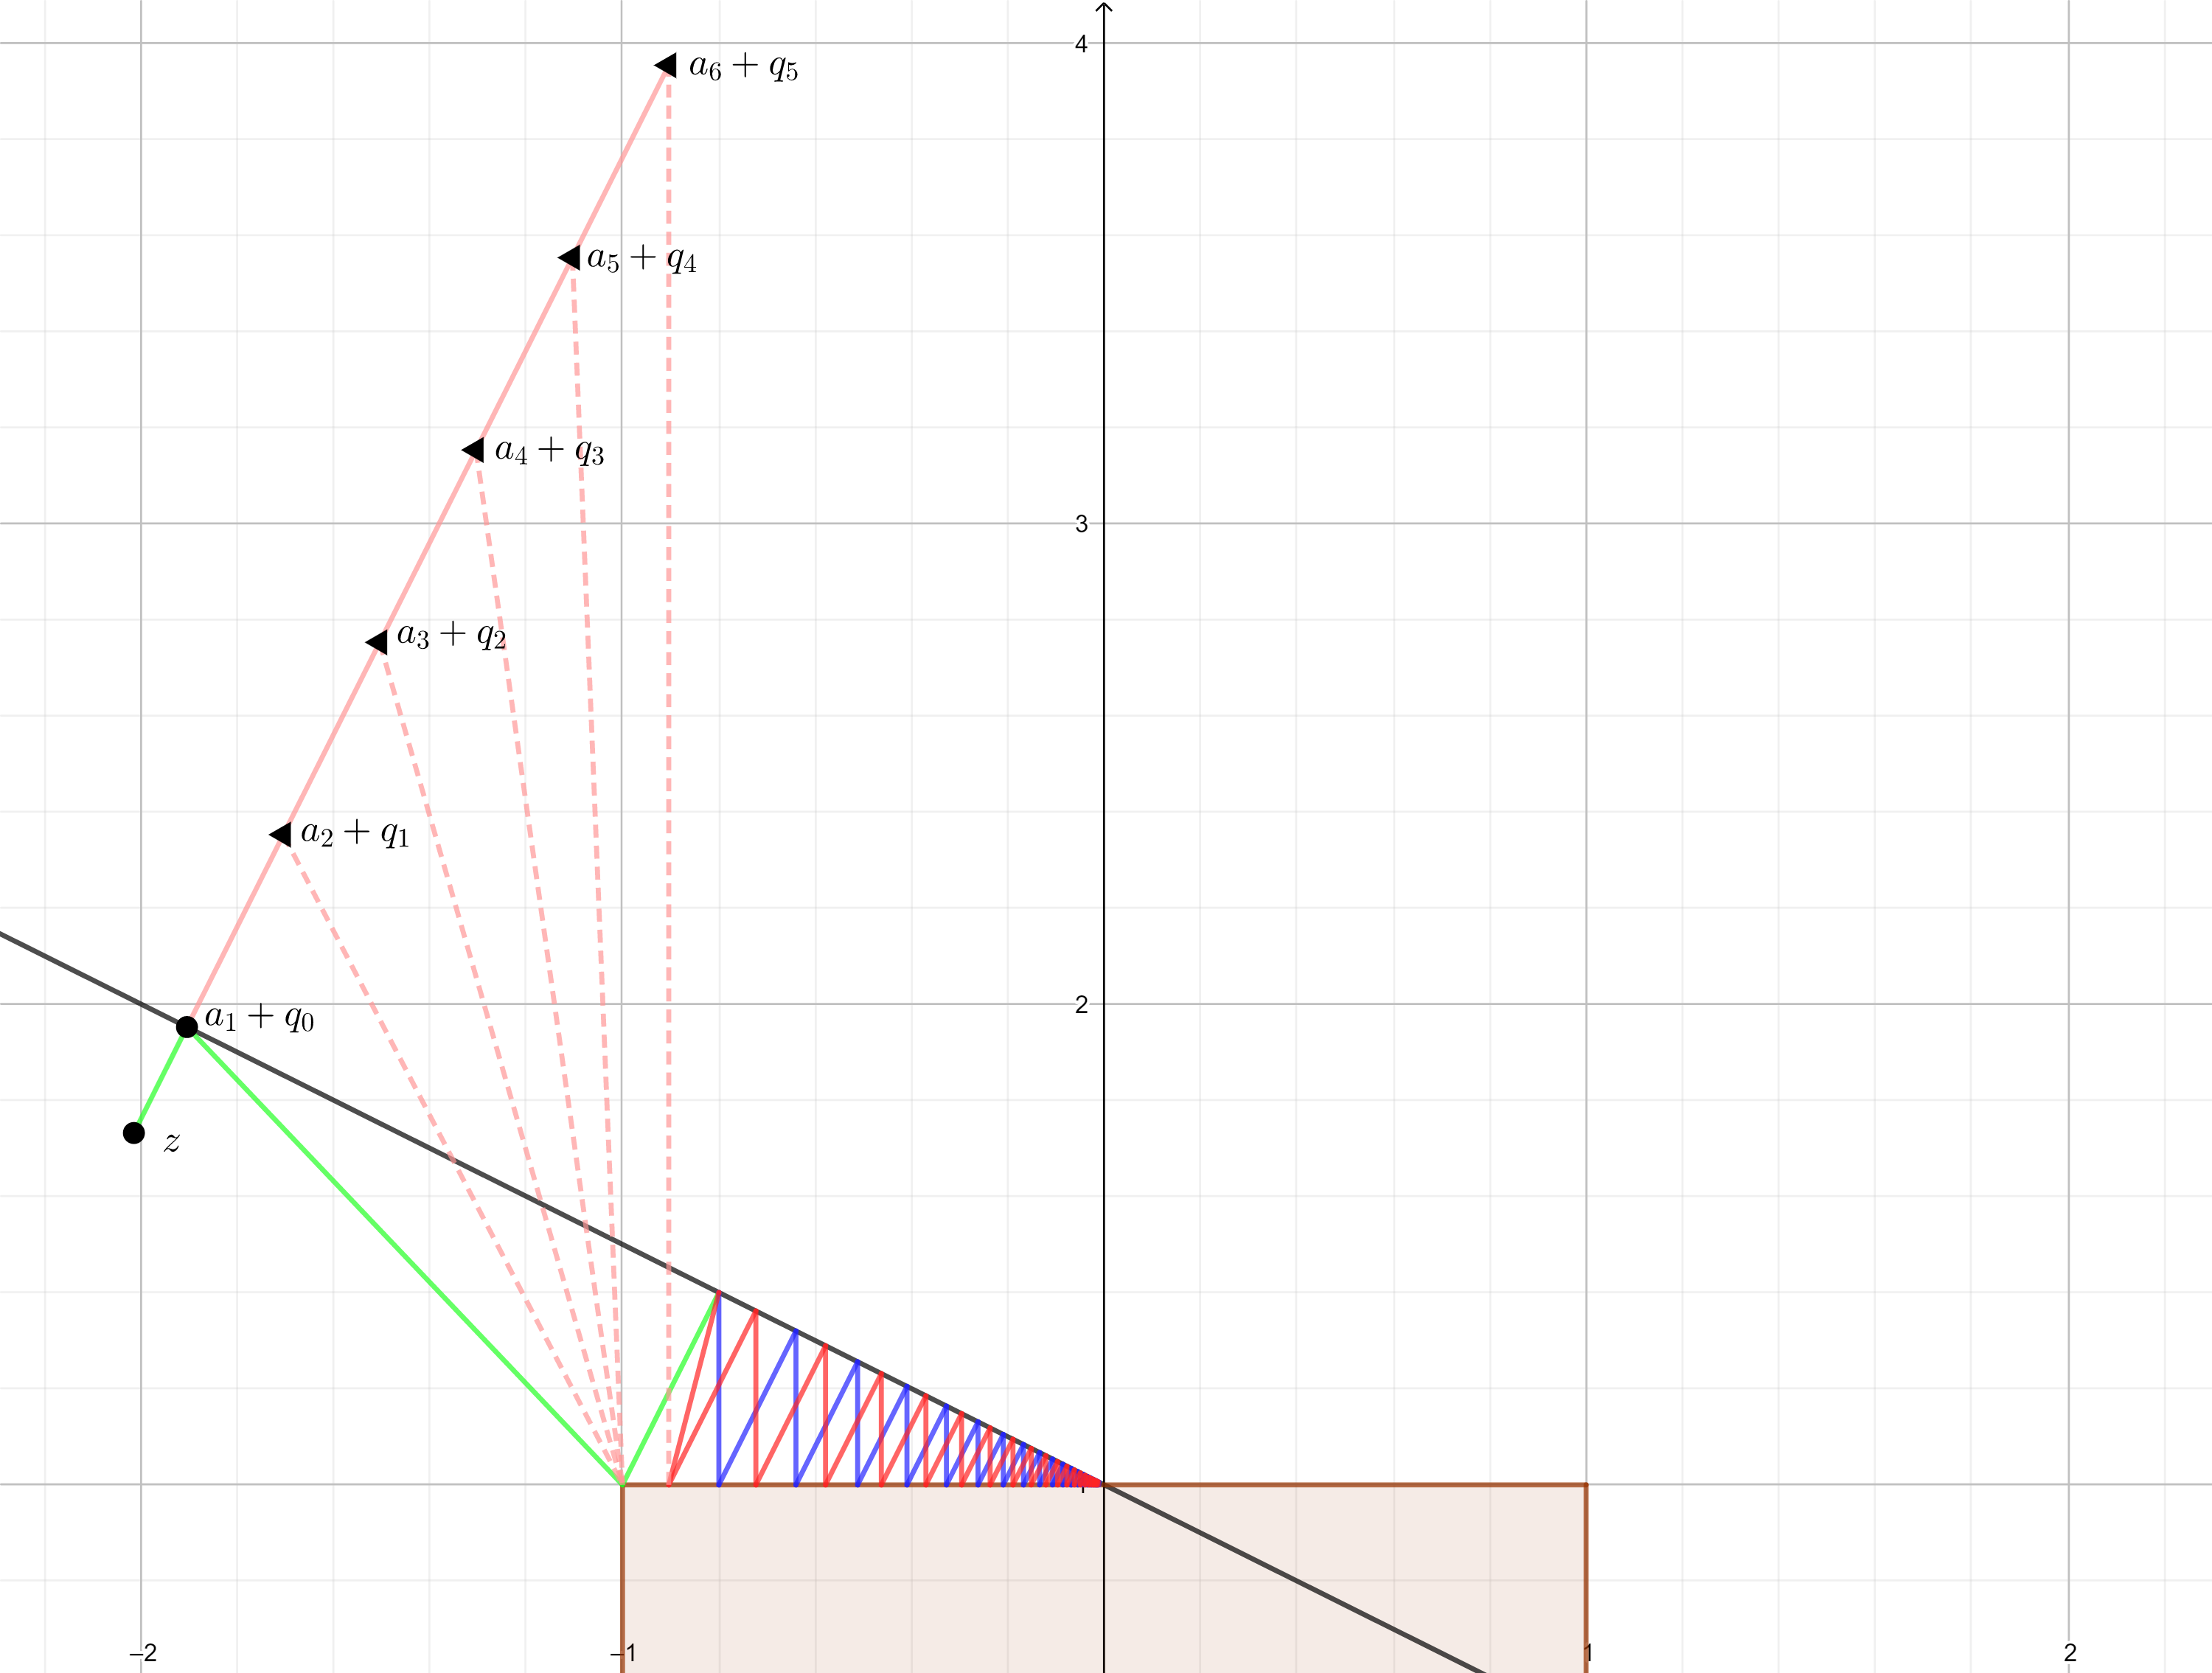
\includegraphics[width=1\textwidth]{Latex/Current Version/Figures/DifferentSequences.png}
        \caption{Stalling for the line-box example when $x_0$ is in the red region.}
        \label{fig:stalling}
    \end{subfigure}
    \caption{A demonstration of the stalling problem for a box and a line. Note how MAP applied to the same constraint sets would not result in any stalling: MAP follows the green line, and subsequently converges via the blue line path.}
    \label{fig:baushkeStall}
\end{figure}
%
\newpage
%
\section{Boundary Smoothness}
% Claudio's contribution
From an analysis of the behaviour of Dykstra's algorithm in the example of Figure~\ref{fig:stalling}, a possible reason behind stalling can be identified in the non-smooth (\cite{SMOOTHNESS}) nature of the boundary of the box's convex set. The algorithm keeps projecting onto the box's corner at the start of each iteration, since this is the closest point to any $x_m$ with $x$ coordinate less than $-1$. This is repeated until $x >= -1$, at which point the algorithm can project onto the top side of the box and exit stalling.
If the boundary of the box was strictly ``smooth'', there would be no corner to get stuck at. The algorithm would get closer to the optimal solution at every step. A non-strict example is illustrated in Figure~\ref{fig:stall}, where the box is rounded by introducing 5 ``rounding corners'' (essentially transforming the box into a solid icosagon).
%
% Figure demonstrating how roundedness prevents stalling
\begin{figure}[h!]
    \centering
    
    \begin{subfigure}[t]{0.49\textwidth}
        \centering
        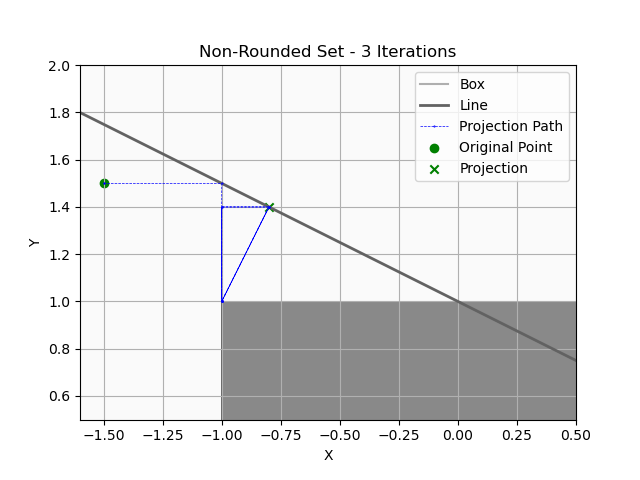
\includegraphics[width=1\textwidth]{Latex/Current Version/Figures/non_rounded_test.png}
        \caption{Dykstra's algorithm on the box and line example}
        \label{fig:nonRounded}
    \end{subfigure}
    \hfill
    \begin{subfigure}[t]{0.49\textwidth}
        \centering
        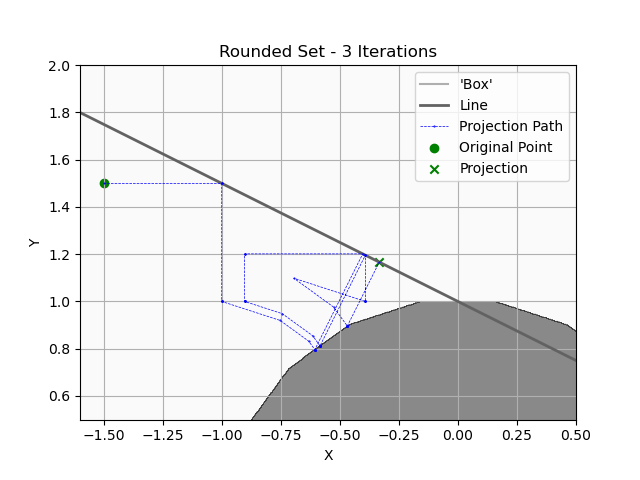
\includegraphics[width=1\textwidth]{Latex/Current Version/Figures/rounded_test.png}
        \caption{Rounded edges prevent algorithm from stalling}
        \label{fig:Rounded}
    \end{subfigure}
    \caption{A demonstration of how roundedness reduces stalling}
    \label{fig:stall}
\end{figure}
%
\par This idea originally seemed to be very promising. However, there are several problems associated with the smoothing out of convex sets' boundaries to prevent stalling:
%
\begin{itemize}
    \item The smoothing adds space and time complexity to the algorithm, both directly and by adding new halfspaces to project upon.
    \item The smoothing may cast the optimal solution onto a non-optimal approximation. This is not the case in our box and line example, but it may represent a serious issue in the MPC implementation.
    \item Most important of all, the added presence of new halfspaces hinders the algorithm's convergence rate. This is further discussed  below.
\end{itemize}
%
Let us consider the same line-box constraint set as~\ref{fig:region}, but now let us place the initial guess at $(-10,~10)$ to increase the count of iterations required to exit stalling. Dykstra's algorithm applied with these conditions, as well as its convergence behaviour, are displayed in Figure~\ref{fig:oneCorner}
%
\begin{figure}[h!]
    \centering
    
    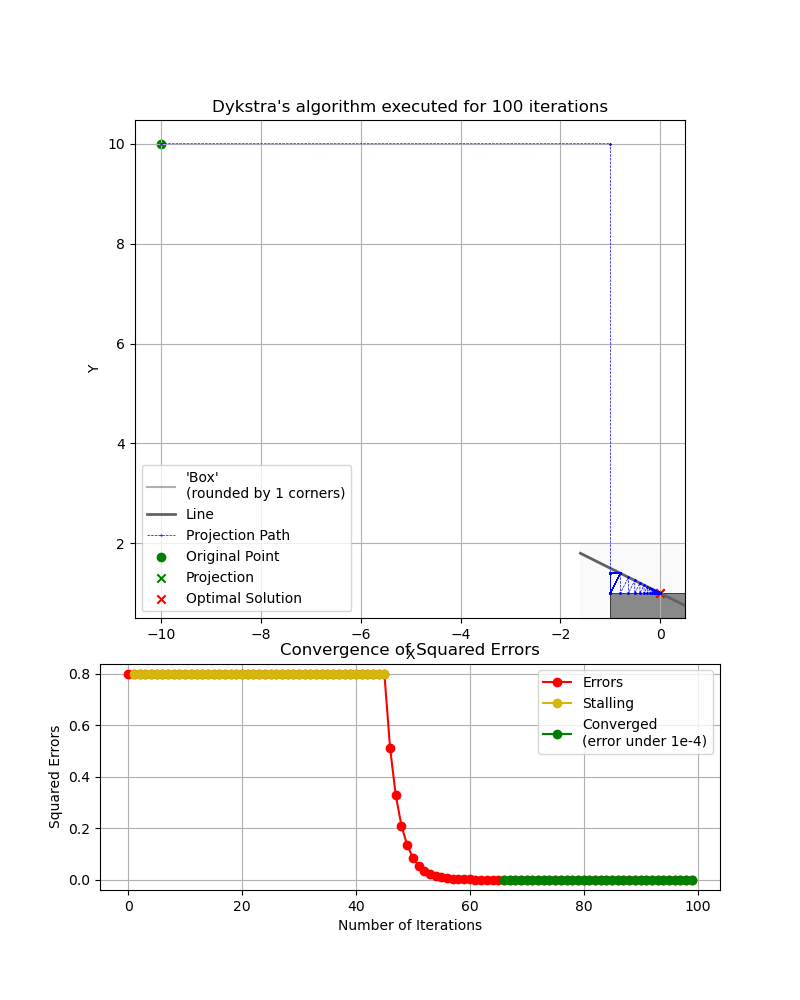
\includegraphics[width=0.6\textwidth]{Latex/Current Version/Figures/one_corner_rounding.png}
    \caption{Dykstra's algorithm applied to initial point $z = (-10,~10)$}
    \label{fig:oneCorner}

\end{figure}
%
\newpage
\par Now compare this to the same box, rounded by 10 corners. The algorithm requires fewer iterations to exit stalling, but convergence is much slower. In this case, the algorithm outputs a much better approximation for the non-rounded set, as shown by comparing Figure~\ref{fig:oneCorner} and Figure~\ref{fig:hundredCorners}.
%
\begin{figure}[h!]
    \centering
    
    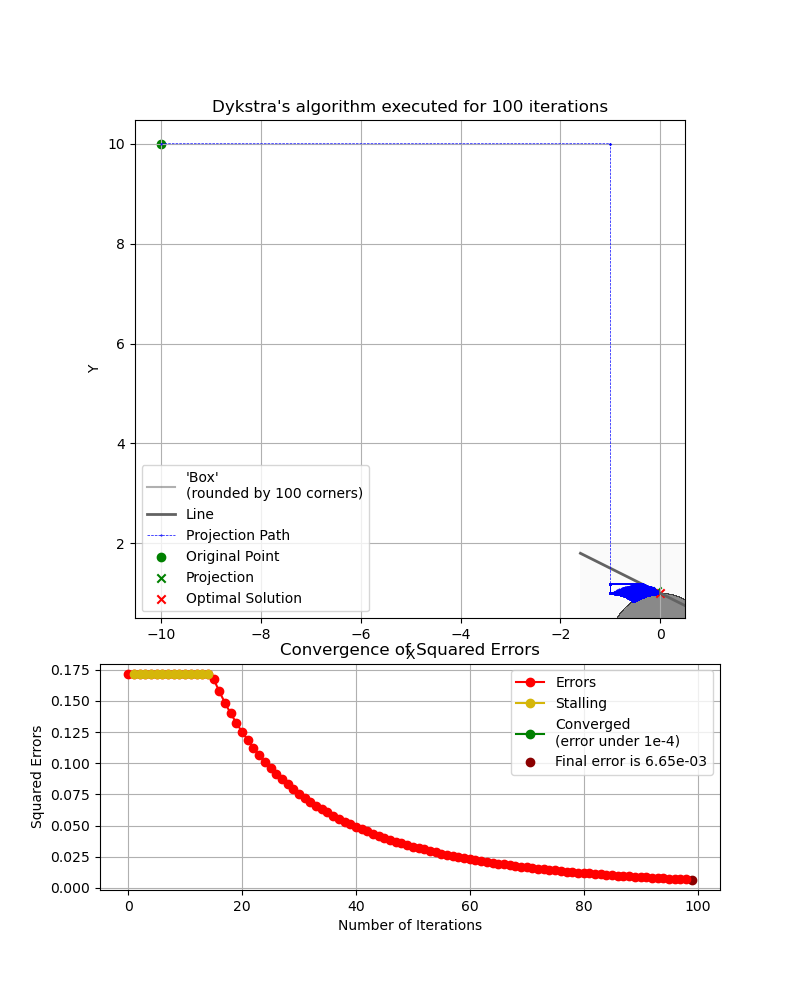
\includegraphics[width=1\textwidth]{Latex/Current Version/Figures/hundred_corners_rounding.png}
    \caption{Dykstra's algorithm applied to initial point $z = (-10, 10)$, box is now rounded by 100 corners}
    \label{fig:hundredCorners}

\end{figure}
\newpage
%
\section{Acceleration for Dykstra's Method}
%
Consider introducing the step size parameter $\beta_m\geq 0$:
\begin{align}\label{eq:dykstramodif}
&x_m=\mathcal{P}_{\mathcal{H}_{[m]}}\left(x_{m-1}+e_{m-n}\right),
&e_m=e_{m-n}+\beta_m(x_{m-1}-x_m).
\end{align}
For $\beta_m=0$, we obtain MAP and for $\beta_m=1$, we obtain Dykstra's method~\eqref{eq:dykstra}. We proceed by characterising the term $e_m$.
\begin{lemma}
It holds that $e_m=y_m f_{[m]}$, where
\begin{align*}
y_n = (1-\beta_m)y_{m-n} +k_m,
\end{align*}
and $k_m=\text{dist}_{\mathcal{H}_{[m]}}(x_{m-1}+e_{m-r})$.
\end{lemma}
\begin{proof}
Suppose that $x_{m-1}+e_{m-n}\in\inter\mathcal{H}_{[m]}$. Then, $x_n=x_{m-1}+e_{m-n}$ and
\begin{align*}
e_m=(1-\beta_m)e_{m-n}.
\end{align*}
Suppose that $x_{m-1}+e_{m-n}\not\in\inter\mathcal{H}_{[m]}$. Then, $x_m=x_{m-1}+e_{m-n}-\left(\iprod{x_{m-1}+e_{m-n}}{f_{[m]}} - c_i\right)f_{[m]}$ and
\begin{align*}
e_m=(1-\beta_m)e_{m-n}+k_mf_{[m]}.
\end{align*}
Note that $e_m=0$ for $m\leq 0$. By induction, $e_m$ is always parallel to $f_{[m]}$ or zero. Substituting $e_m=y_nf_{[m]}$ yields
\begin{align*}
y_m=(1-\beta_m)y_{m-n}+k_m.
\end{align*} 
\end{proof}
%
The introduction of $\beta_m$ adds another degree of freedom to Dykstra's algorithm. This parameter could be chosen before the algorithm is applied, or even before each iteration. How to compute an optimal choice of $\beta_m$ is currently under investigation.
%
\newpage
\par For our beloved line-box example with starting choice of $z = (-10,~10)$, it is easy to spot how a choice of $\beta_m = 0$ would be optimal. The algorithm would converge as shown in Figure~\ref{fig:MAPtenten}
%
\begin{figure}[h!]
    \centering
    
    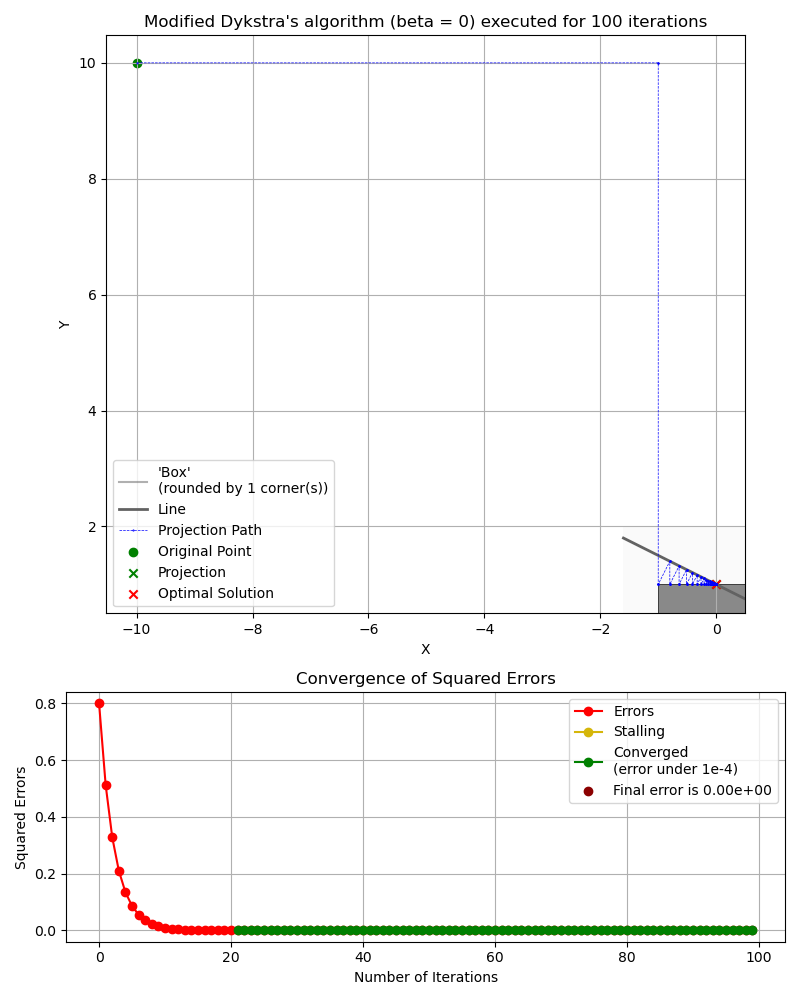
\includegraphics[width=1\textwidth]{Latex/Current Version/Figures/MAP_one_corner.png}
    \caption{Dykstra's algorithm applied to initial point $z = (-10,~10)$, with $\beta_m = 0$. This is essentially applying MAP}
    \label{fig:MAPtenten}

\end{figure}
%
\section{Choice of $\beta_m$} \label{sec: new algorithm}
%
As discussed in Section~\ref{sec: dykstra}, MAP does not always produce the optimal solution as its output. In general, MAP will converge weakly to \textit{some} point on the feasible region (i.e. locus of points which constitute the intersection of all halfspaces)~\cite{BREGMAN}. More specifically, if $x_m \in \bigcap_{i=1}^n \mathcal{H}_i$, then $x_{m+1},~x_{m+2},~... = x_m$. This constitutes MAP's biggest flaw, as seen in Figure~\ref{fig:MAPterminates}.
%
\begin{figure}[h!]
    \centering
    
    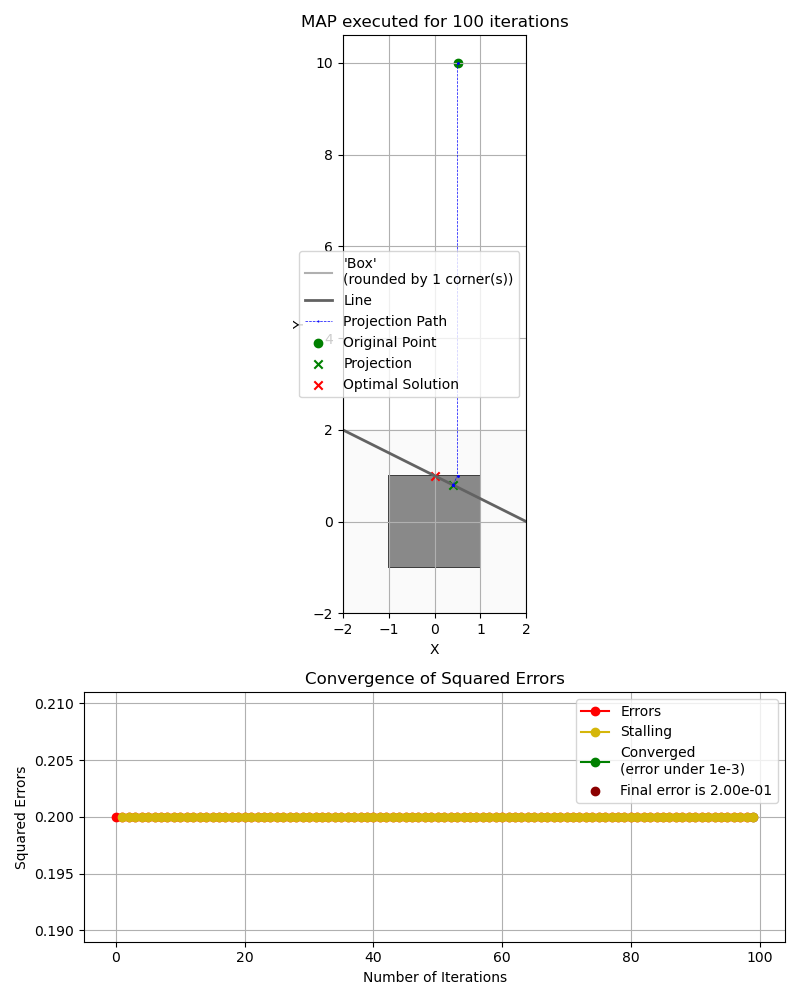
\includegraphics[width=0.95\textwidth]{Latex/Current Version/Figures/in_intersection_MAP.png}
    \caption{MAP applied to initial point $z = (0.5,~10)$. We land on a point on the intersection of all halfspaces on first iteration, hence algorithm does not proceed any further}
    \label{fig:MAPterminates}

\end{figure}
%
\newpage
However, when the initial point to be projected lies outside of $\bigcap_{i=1}^n \mathcal{H}_i$, and if $x_m \notin \bigcap_{i=1}^n \mathcal{H}_i \forall m$, then MAP will not stall and the series of iterates produced by MAP and Dykstra's method coincide, with infinite convergence (at least in this line and box example, but I think this can be generalised).
\par It follows that, if we combine the non-stalling nature of MAP with the certainty of producing an optimal solution of Dykstra's method, we could altogether avoid stalling. This is how we have decided to choose parameter $\beta_m$:
%
\begin{enumerate}
\item $\beta_0$ is initialised to $1$
\item At the start of each iteration, if $x_m \notin \bigcap_{i=1}^n \mathcal{H}_i$, then $\beta_{m+1}$ is set to $0$, employing MAP for the next iteration.
\item Otherwise, $\beta_{m+1}$ is set to $1$, employing Dykstra's method instead
\end{enumerate}
%
\par This simple modification will ensure we do not stall even if we are arbitrarily deep into the red region, and also that we will not terminate if at any point we land in the feasible region. It is important to note that, in order for this to work, we still have to \textit{keep track} of the sequence of errors $e_m$ we would obtain using Dykstra's algorithm, in case we need to use them in the next iteration. The improvements brought forward by this modification are highlighted in Figure~\ref{fig:oneCornerModified} (compare this to Figure~\ref{fig:oneCorner}).
%
\begin{figure}[h!]
    \centering
    
    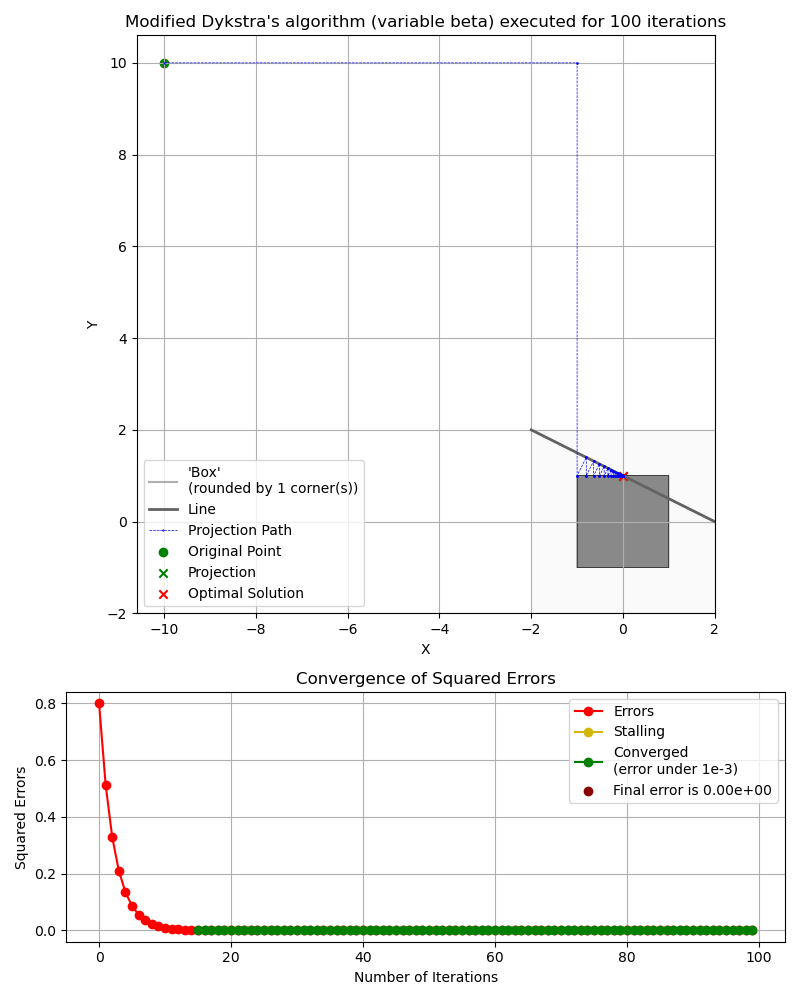
\includegraphics[width=0.6\textwidth]{Latex/Current Version/Figures/not_in_intersection_modified.png}
    \caption{Modified method applied to initial point $z = (-10,~10)$.}
    \label{fig:oneCornerModified}

\end{figure}
%
\newpage
It is also worth remarking that this new modified algorithm will also work in the circumstance where we land in the intersection at some point $x_m$. Compare Figure~\ref{fig:MAPterminates} to Figure~\ref{fig:noTermination} below:
%
\begin{figure}[h!]
    \centering
    
    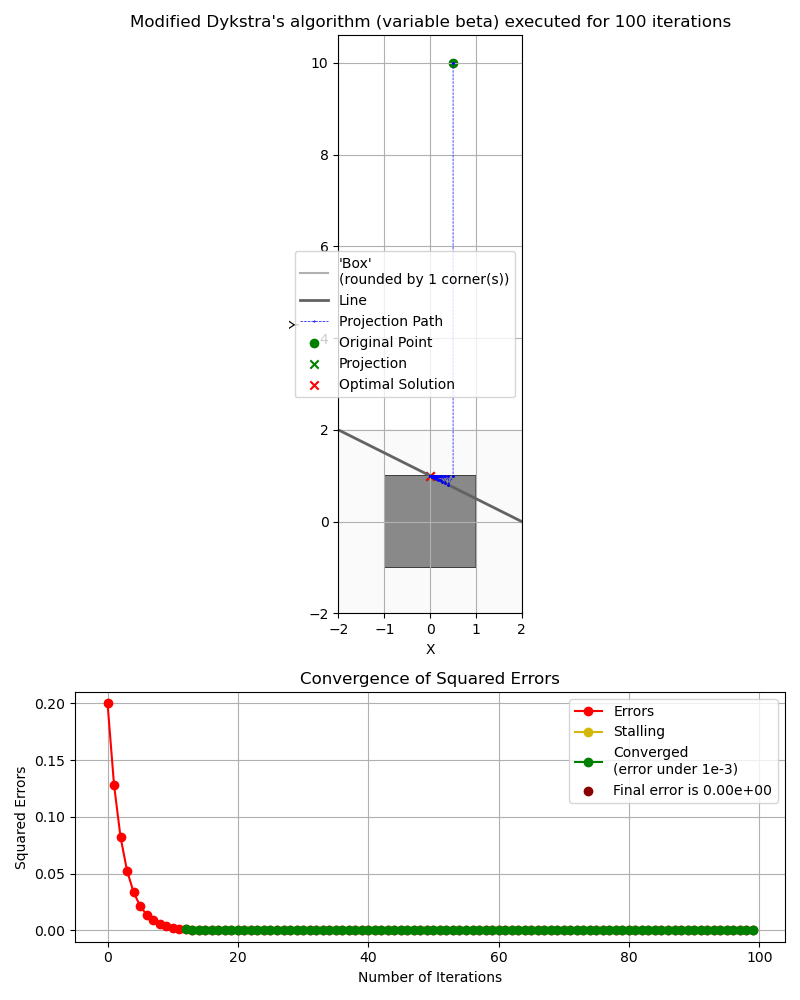
\includegraphics[width=1\textwidth]{Latex/Current Version/Figures/in_intersection_modified.png}
    \caption{Modified method applied to initial point $z = (0.5,~10)$. In this case, $\beta_m$ is set to $1$ for all $m > 1$.}
    \label{fig:noTermination}

\end{figure}
%
\section{Thoughts}
%
It seems that the modified algorithm proposed in Section~\ref{sec: new algorithm} is able to completely avoid stalling in the line-box example proposed by Bauschke. We have implemented a new parameter $\beta_m$, which allows us to choose between MAP and Dykstra's method based on the current projection $x_m$. This new algorithm demonstrates at worst infinite convergence with no stalling, for any $\inRv{z}{2}$, which constitutes a drastic improvement compared to the results of Figure~\ref{fig:region}.
\par If we assume that MAP cannot stall (which follows intuition for convex sets), then to demonstrate our algorithm never stalls it would be sufficient to prove that \emph{any intermediate step $x_m$ which lies in the feasible region cannot lead to stalling} (note how an initial point $z \in \bigcap_{i=1}^n \mathcal{H}_i$ already constitutes the optimal solution). See Figure~\ref{fig:intermediates} for a practical example. This should cast our initial problem into a much more confined one.
%
\begin{figure}[h!]
    \centering
    
    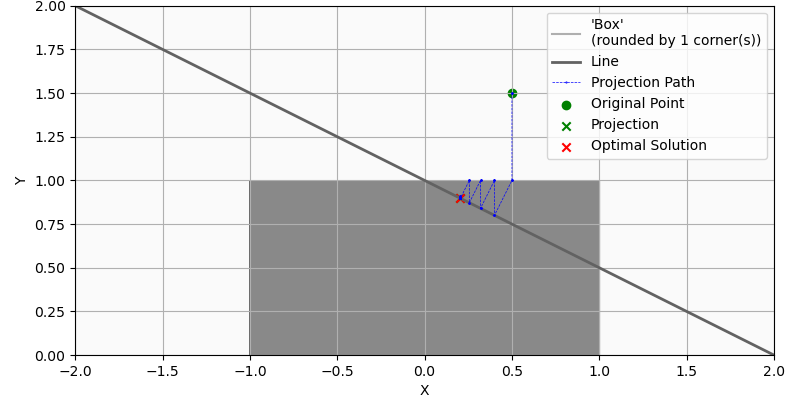
\includegraphics[width=1\textwidth]{Latex/Current Version/Figures/intermediate_steps.png}
    \caption{In an example such as this one, to show no stalling, one would have to prove that, if we land on one of the blue dots within the feasible region (line segment between $(0,~1)$ and $(1,~0.5)$), then it is not possible to stall.}
    \label{fig:intermediates}

\end{figure}
%
\par However, some questions still remain unanswered:
\begin{itemize}
\item Can we generalise the algorithm outlined in Section~\ref{sec: new algorithm} to work with any choice of halfspaces and in any number of dimensions?
\item The new algorithm requires we check every halfspace at the start of each iteration, which is expensive: can we keep track of which halfspaces remain active, and only check those to obtain a value of $\beta_{m+1}$?
\item Is there any value in rounding the edges of our constraint sets?
\item Can Dysktra's method be accelerated after escaping the stalling region (e.g. by choosing a value of $\beta_m \neq 1$)?
\end{itemize}
%
% References
\newpage
\bibliographystyle{plain}
\bibliography{master_bib_abbrev}

\end{document}